\chapter{Security} \label{security}

During the development of Skylab, security has always been a priority. Common attacks such as SQL injection, XSS attacks and CSRF attacks are all addressed by the Rails framework itself. Skylab's main security focus is to make sure authentication process and access control are well-defined and can withstand various attacks.

\section{User authentication}

There are basically 2 ways to login to Skylab: email and password combination and NUS OpenID. For email and password combination, we employ Devise to manage authentication related information in \textit{User} model. Devise has been used widely in Rails community and currently there are more than 13,000 stars of Devise repository on GitHub\cite{citationdevise}. What is more, according to security scanning of Devise by Hakiri there is no security warning, which further proves the trust-ability of Devise\cite{citationdevisehakiri}. As for NUS OpenID, it is using OAuth 2.0 as authentication protocol, which is believed to be safe and currently is adopted by many OpenID providers as well\cite{citationnusopenid}.

\section{Access control}

Skylab is adopting role based access control strategy to grant different permissions for different users. There are basically 4 levels of checking for each incoming requests:

\begin{itemize}
  \item \textbf{login\_required:} a boolean value. If a action is login\_required then a user must sign to be granted for the access.
  \item \textbf{admin\_only:} a boolean value. If a action is admin\_only then only users with role of \textit{Admin} can access; but if current user is admin, the next check will be skipped and return true directly as admin users can access any resources in Skylab.
  \item \textbf{allowed\_users:} a boolean value. If a action requires login and is not only accessed by admins, then the current logged-in user will be checked against the list of allowed users who have the permissions.
  \item \textbf{strategy:} a lambda function which can be executed and is expected to return a boolean value. If the lambda is provided by the caller, it will be executed and whether users in allowed\_users can actually access the resource or not depends on the returned result.
\end{itemize}

As this checking procedure is a common to nearly all actions, it is defined in \textit{ApplicationController} which will be effectively inherited by all controllers in Skylab. So all methods in those controllers can invoke this method to check user's permission first.

\section{Security warnings}

Hakiri is used as the security analysis tool in Skylab. Currently there are some warnings in cross-site scripting, code injection, file access, input validation, resource management according to Hakiri scanning result. However, all of these security issues are actually vulnerabilities in current version of Ruby on Rails framework used by Skylab --- so this means that by upgrading the Rails framework we can simply remove these issues.

\begin{figure}[h]
	\centering
	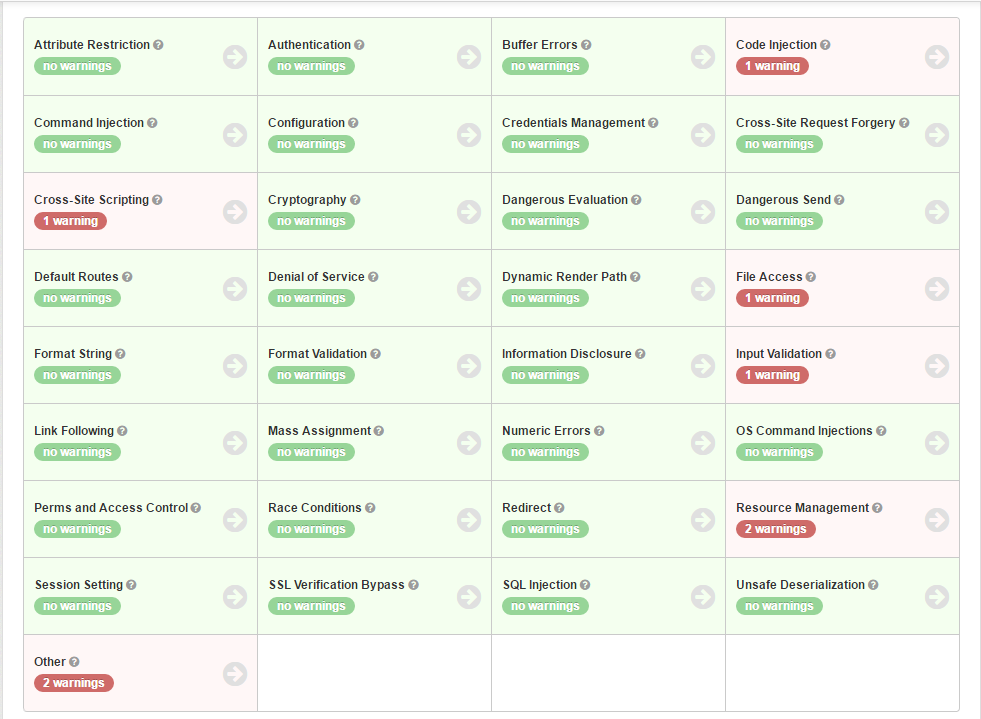
\includegraphics[width=\textwidth]{Images/Skylab_Hakiri.png}
	\caption{Hakiri security warnings}
	\label{fig:SkylabHakiri}
\end{figure}

Due the importance of security in the development of a web application, security will remain as an prioritized task in Skylab and more future work will be done regarding this as well.
